% !TEX root = ../../main.tex

\section{Getting responses from the \acrshort{api}} % (fold)
\label{sec:getting_responses_from_the_api}

Until now, all state operations only applied to the local view, but no \acrshort{api} calls have been made. Since Algolia queries are called via its \acrshort{api}, it's very important that these \acrshort{api} calls will happen as soon as something in the query state changes. 

A subscription to the main state is made to make sure that every time the state changes, a new \acrshort{api} request can be done. Once this request fulfils, a function called {\tt \_\_setResults} can be called with the new values that are returned from the API.

To be able to use the refinements smoothly, a transformation needs to happen before setting those results as actual state. Every type of refinement has a function called {\tt mapResponseToState}. This function will be called for each of the existing types of refinements in the current state.

\begin{figure}[H]
  \centering
  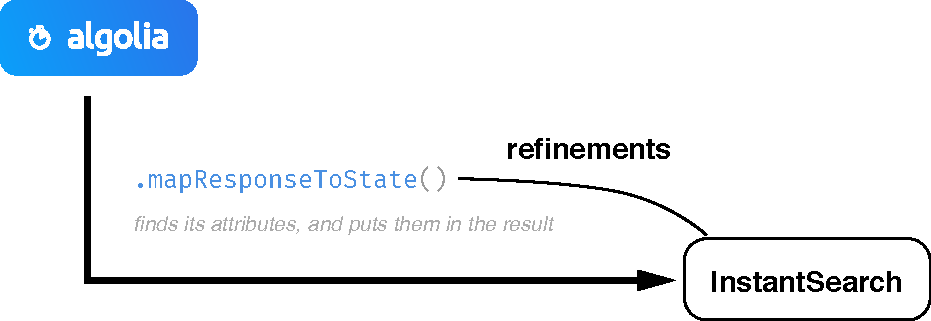
\includegraphics[width=0.8\textwidth]{results-to-state.pdf}
  \caption{Mapping \acrshort{api} responses to InstantSearch state}
  \label{figure:results-to-state}
\end{figure}

% section getting_responses_from_the_api (end)
